\PassOptionsToPackage{unicode=true}{hyperref} % options for packages loaded elsewhere
\PassOptionsToPackage{hyphens}{url}
%
\documentclass[]{article}
\usepackage{lmodern}
\usepackage{amssymb,amsmath}
\usepackage{ifxetex,ifluatex}
\usepackage{fixltx2e} % provides \textsubscript
\ifnum 0\ifxetex 1\fi\ifluatex 1\fi=0 % if pdftex
  \usepackage[T1]{fontenc}
  \usepackage[utf8]{inputenc}
  \usepackage{textcomp} % provides euro and other symbols
\else % if luatex or xelatex
  \usepackage{unicode-math}
  \defaultfontfeatures{Ligatures=TeX,Scale=MatchLowercase}
\fi
% use upquote if available, for straight quotes in verbatim environments
\IfFileExists{upquote.sty}{\usepackage{upquote}}{}
% use microtype if available
\IfFileExists{microtype.sty}{%
\usepackage[]{microtype}
\UseMicrotypeSet[protrusion]{basicmath} % disable protrusion for tt fonts
}{}
\IfFileExists{parskip.sty}{%
\usepackage{parskip}
}{% else
\setlength{\parindent}{0pt}
\setlength{\parskip}{6pt plus 2pt minus 1pt}
}
\usepackage{hyperref}
\hypersetup{
            pdftitle={Project 2: Modeling, Testing, and Predicting},
            pdfauthor={Alexandra Sears},
            pdfborder={0 0 0},
            breaklinks=true}
\urlstyle{same}  % don't use monospace font for urls
\usepackage[margin=1in]{geometry}
\usepackage{color}
\usepackage{fancyvrb}
\newcommand{\VerbBar}{|}
\newcommand{\VERB}{\Verb[commandchars=\\\{\}]}
\DefineVerbatimEnvironment{Highlighting}{Verbatim}{commandchars=\\\{\}}
% Add ',fontsize=\small' for more characters per line
\usepackage{framed}
\definecolor{shadecolor}{RGB}{248,248,248}
\newenvironment{Shaded}{\begin{snugshade}}{\end{snugshade}}
\newcommand{\AlertTok}[1]{\textcolor[rgb]{0.94,0.16,0.16}{#1}}
\newcommand{\AnnotationTok}[1]{\textcolor[rgb]{0.56,0.35,0.01}{\textbf{\textit{#1}}}}
\newcommand{\AttributeTok}[1]{\textcolor[rgb]{0.77,0.63,0.00}{#1}}
\newcommand{\BaseNTok}[1]{\textcolor[rgb]{0.00,0.00,0.81}{#1}}
\newcommand{\BuiltInTok}[1]{#1}
\newcommand{\CharTok}[1]{\textcolor[rgb]{0.31,0.60,0.02}{#1}}
\newcommand{\CommentTok}[1]{\textcolor[rgb]{0.56,0.35,0.01}{\textit{#1}}}
\newcommand{\CommentVarTok}[1]{\textcolor[rgb]{0.56,0.35,0.01}{\textbf{\textit{#1}}}}
\newcommand{\ConstantTok}[1]{\textcolor[rgb]{0.00,0.00,0.00}{#1}}
\newcommand{\ControlFlowTok}[1]{\textcolor[rgb]{0.13,0.29,0.53}{\textbf{#1}}}
\newcommand{\DataTypeTok}[1]{\textcolor[rgb]{0.13,0.29,0.53}{#1}}
\newcommand{\DecValTok}[1]{\textcolor[rgb]{0.00,0.00,0.81}{#1}}
\newcommand{\DocumentationTok}[1]{\textcolor[rgb]{0.56,0.35,0.01}{\textbf{\textit{#1}}}}
\newcommand{\ErrorTok}[1]{\textcolor[rgb]{0.64,0.00,0.00}{\textbf{#1}}}
\newcommand{\ExtensionTok}[1]{#1}
\newcommand{\FloatTok}[1]{\textcolor[rgb]{0.00,0.00,0.81}{#1}}
\newcommand{\FunctionTok}[1]{\textcolor[rgb]{0.00,0.00,0.00}{#1}}
\newcommand{\ImportTok}[1]{#1}
\newcommand{\InformationTok}[1]{\textcolor[rgb]{0.56,0.35,0.01}{\textbf{\textit{#1}}}}
\newcommand{\KeywordTok}[1]{\textcolor[rgb]{0.13,0.29,0.53}{\textbf{#1}}}
\newcommand{\NormalTok}[1]{#1}
\newcommand{\OperatorTok}[1]{\textcolor[rgb]{0.81,0.36,0.00}{\textbf{#1}}}
\newcommand{\OtherTok}[1]{\textcolor[rgb]{0.56,0.35,0.01}{#1}}
\newcommand{\PreprocessorTok}[1]{\textcolor[rgb]{0.56,0.35,0.01}{\textit{#1}}}
\newcommand{\RegionMarkerTok}[1]{#1}
\newcommand{\SpecialCharTok}[1]{\textcolor[rgb]{0.00,0.00,0.00}{#1}}
\newcommand{\SpecialStringTok}[1]{\textcolor[rgb]{0.31,0.60,0.02}{#1}}
\newcommand{\StringTok}[1]{\textcolor[rgb]{0.31,0.60,0.02}{#1}}
\newcommand{\VariableTok}[1]{\textcolor[rgb]{0.00,0.00,0.00}{#1}}
\newcommand{\VerbatimStringTok}[1]{\textcolor[rgb]{0.31,0.60,0.02}{#1}}
\newcommand{\WarningTok}[1]{\textcolor[rgb]{0.56,0.35,0.01}{\textbf{\textit{#1}}}}
\usepackage{graphicx,grffile}
\makeatletter
\def\maxwidth{\ifdim\Gin@nat@width>\linewidth\linewidth\else\Gin@nat@width\fi}
\def\maxheight{\ifdim\Gin@nat@height>\textheight\textheight\else\Gin@nat@height\fi}
\makeatother
% Scale images if necessary, so that they will not overflow the page
% margins by default, and it is still possible to overwrite the defaults
% using explicit options in \includegraphics[width, height, ...]{}
\setkeys{Gin}{width=\maxwidth,height=\maxheight,keepaspectratio}
\setlength{\emergencystretch}{3em}  % prevent overfull lines
\providecommand{\tightlist}{%
  \setlength{\itemsep}{0pt}\setlength{\parskip}{0pt}}
\setcounter{secnumdepth}{0}
% Redefines (sub)paragraphs to behave more like sections
\ifx\paragraph\undefined\else
\let\oldparagraph\paragraph
\renewcommand{\paragraph}[1]{\oldparagraph{#1}\mbox{}}
\fi
\ifx\subparagraph\undefined\else
\let\oldsubparagraph\subparagraph
\renewcommand{\subparagraph}[1]{\oldsubparagraph{#1}\mbox{}}
\fi

% set default figure placement to htbp
\makeatletter
\def\fps@figure{htbp}
\makeatother

\usepackage{booktabs}
\usepackage{longtable}
\usepackage{array}
\usepackage{multirow}
\usepackage{wrapfig}
\usepackage{float}
\usepackage{colortbl}
\usepackage{pdflscape}
\usepackage{tabu}
\usepackage{threeparttable}
\usepackage{threeparttablex}
\usepackage[normalem]{ulem}
\usepackage{makecell}
\usepackage{xcolor}

\title{Project 2: Modeling, Testing, and Predicting}
\author{Alexandra Sears}
\date{4/1/2020}

\begin{document}
\maketitle

\begin{Shaded}
\begin{Highlighting}[]
\NormalTok{jasa<-survival}\OperatorTok{::}\NormalTok{jasa}
\NormalTok{jasa<-jasa}\OperatorTok\KeywordTok{select}\NormalTok{(fustat,age,reject,surgery,accept.dt,tx.date,wait.time)}\OperatorTok
\StringTok{  }\NormalTok{na.omit}\OperatorTok\KeywordTok{mutate}\NormalTok{(}\DataTypeTok{survive=}\NormalTok{fustat)}\OperatorTok\KeywordTok{select}\NormalTok{(}\OperatorTok{-}\NormalTok{fustat)}
\KeywordTok{glimpse}\NormalTok{(jasa)}
\end{Highlighting}
\end{Shaded}

\begin{verbatim}
## Rows: 65
## Columns: 7
## $ age       <dbl> 54.29706, 40.26283, 50.86927, 42.50240, 47.98084, 54.5735...
## $ reject    <dbl> 0, 0, 1, 1, 0, 1, 1, 1, 0, 1, 1, 1, 1, 1, 0, 0, 1, 1, 0, ...
## $ surgery   <dbl> 0, 0, 0, 0, 0, 0, 0, 0, 0, 0, 0, 0, 0, 0, 0, 0, 0, 0, 0, ...
## $ accept.dt <date> 1968-01-06, 1968-03-28, 1968-07-12, 1968-08-11, 1968-08-...
## $ tx.date   <date> 1968-01-06, 1968-05-02, 1968-08-31, 1968-08-22, 1968-09-...
## $ wait.time <dbl> 0, 35, 50, 11, 25, 16, 36, 27, 19, 17, 7, 11, 2, 82, 24, ...
## $ survive   <dbl> 1, 1, 1, 1, 1, 1, 1, 1, 1, 1, 1, 1, 1, 1, 0, 1, 1, 1, 0, ...
\end{verbatim}

\hypertarget{introduction}{%
\paragraph{0. Introduction}\label{introduction}}

\emph{The data set is the survival of patients on the waiting list for a
Stanford heart transplant program in 1974 that was published by John
Crowley \& Marie Hu{[}1{]}. Survive is if the patient survived with 1
being that they died. Age is the age of the patient in years. Reject is
whether or not they rejected the transplant with 1 being they did.
Surgery is if the had a prior bypass surgery with 1 being they did.
accept.dt and tx.dt are the acceptance into the program and the date of
the transplant respectively. wait.time is the time before the pateint
had the transplant (which is just days between accept.dt and
tx.date).There are 65 observations after removing the NAs.}

\hypertarget{manova-anova-post-hoc-t-tests}{%
\paragraph{1. MANOVA, ANOVA, Post-Hoc t
Tests}\label{manova-anova-post-hoc-t-tests}}

\begin{Shaded}
\begin{Highlighting}[]
\KeywordTok{shapiro.test}\NormalTok{(jasa}\OperatorTok{$}\NormalTok{age)}
\end{Highlighting}
\end{Shaded}

\begin{verbatim}
## 
##  Shapiro-Wilk normality test
## 
## data:  jasa$age
## W = 0.93631, p-value = 0.002338
\end{verbatim}

\begin{Shaded}
\begin{Highlighting}[]
\KeywordTok{shapiro.test}\NormalTok{(jasa}\OperatorTok{$}\NormalTok{reject)}
\end{Highlighting}
\end{Shaded}

\begin{verbatim}
## 
##  Shapiro-Wilk normality test
## 
## data:  jasa$reject
## W = 0.63232, p-value = 1.738e-11
\end{verbatim}

\begin{Shaded}
\begin{Highlighting}[]
\KeywordTok{shapiro.test}\NormalTok{(jasa}\OperatorTok{$}\NormalTok{surgery)}
\end{Highlighting}
\end{Shaded}

\begin{verbatim}
## 
##  Shapiro-Wilk normality test
## 
## data:  jasa$surgery
## W = 0.47225, p-value = 6.437e-14
\end{verbatim}

\begin{Shaded}
\begin{Highlighting}[]
\KeywordTok{shapiro.test}\NormalTok{(jasa}\OperatorTok{$}\NormalTok{wait.time)}
\end{Highlighting}
\end{Shaded}

\begin{verbatim}
## 
##  Shapiro-Wilk normality test
## 
## data:  jasa$wait.time
## W = 0.63669, p-value = 2.071e-11
\end{verbatim}

\begin{Shaded}
\begin{Highlighting}[]
\NormalTok{jasa}\OperatorTok\StringTok{ }\KeywordTok{select}\NormalTok{(age,reject,surgery,wait.time)}\OperatorTok\NormalTok{cor}
\end{Highlighting}
\end{Shaded}

\begin{verbatim}
##                   age     reject     surgery   wait.time
## age        1.00000000  0.4289776 -0.02497560  0.01183281
## reject     0.42897762  1.0000000 -0.18776413 -0.19880603
## surgery   -0.02497560 -0.1877641  1.00000000  0.05814853
## wait.time  0.01183281 -0.1988060  0.05814853  1.00000000
\end{verbatim}

\begin{Shaded}
\begin{Highlighting}[]
\NormalTok{df<-}\KeywordTok{rmvnorm}\NormalTok{(}\DecValTok{1000}\NormalTok{,}\DataTypeTok{mean=}\KeywordTok{c}\NormalTok{(}\DecValTok{0}\NormalTok{,}\DecValTok{0}\NormalTok{),}\DataTypeTok{sigma=}\KeywordTok{matrix}\NormalTok{(}\KeywordTok{c}\NormalTok{(}\DecValTok{1}\NormalTok{,.}\DecValTok{5}\NormalTok{,.}\DecValTok{5}\NormalTok{,}\DecValTok{1}\NormalTok{),}\DataTypeTok{ncol=}\DecValTok{2}\NormalTok{,}\DataTypeTok{byrow=}\NormalTok{T))}
\NormalTok{df<-}\KeywordTok{data.frame}\NormalTok{(jasa)}\OperatorTok\KeywordTok{rename}\NormalTok{(}\DataTypeTok{Y1=}\NormalTok{survive,}\DataTypeTok{Y2=}\NormalTok{age)}
\NormalTok{p<-}\KeywordTok{ggplot}\NormalTok{(df, }\KeywordTok{aes}\NormalTok{(Y1,Y2))}\OperatorTok{+}\KeywordTok{theme_classic}\NormalTok{()}\OperatorTok{+}\KeywordTok{xlim}\NormalTok{(}\OperatorTok{-}\DecValTok{10}\NormalTok{, }\DecValTok{10}\NormalTok{)}\OperatorTok{+}\KeywordTok{geom_point}\NormalTok{(}\DataTypeTok{alpha=}\NormalTok{.}\DecValTok{5}\NormalTok{)}\OperatorTok{+}\KeywordTok{geom_density_2d}\NormalTok{(}\DataTypeTok{h=}\DecValTok{2}\NormalTok{)}\OperatorTok{+}\KeywordTok{coord_fixed}\NormalTok{()}
\KeywordTok{ggMarginal}\NormalTok{(p,}\DataTypeTok{type=}\StringTok{"density"}\NormalTok{,}\DataTypeTok{xparams =} \KeywordTok{list}\NormalTok{(}\DataTypeTok{bw=}\NormalTok{.}\DecValTok{5}\NormalTok{), }\DataTypeTok{yparams=}\KeywordTok{list}\NormalTok{(}\DataTypeTok{bw=}\NormalTok{.}\DecValTok{5}\NormalTok{))}
\end{Highlighting}
\end{Shaded}

\begin{center}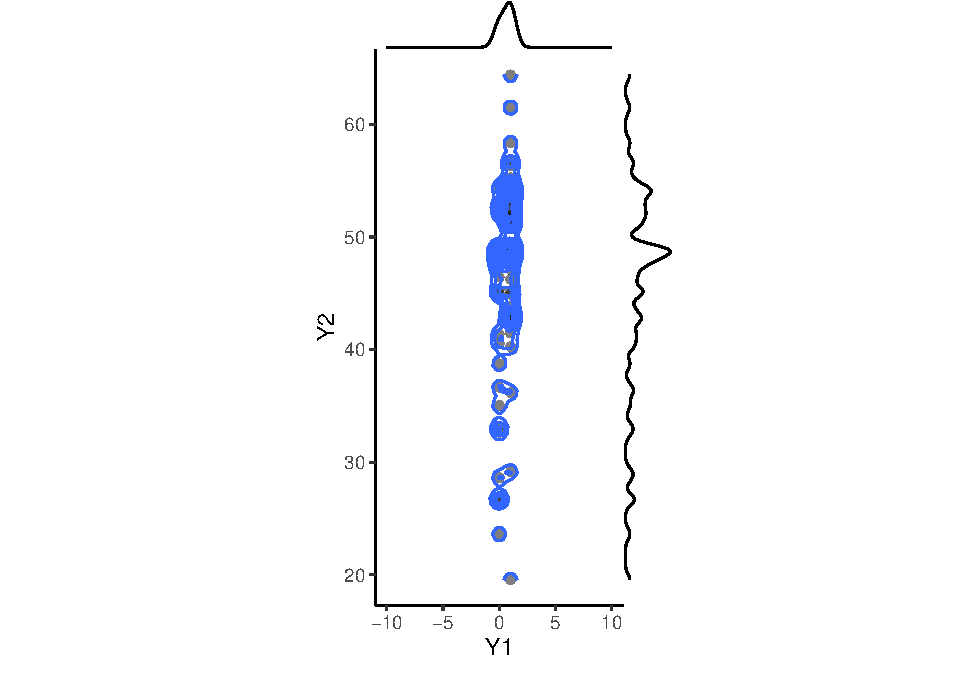
\includegraphics{proj2-2_files/figure-latex/unnamed-chunk-2-1} \end{center}

\begin{Shaded}
\begin{Highlighting}[]
\KeywordTok{ggplot}\NormalTok{(jasa, }\KeywordTok{aes}\NormalTok{(}\DataTypeTok{x =}\NormalTok{ age, }\DataTypeTok{y =}\NormalTok{ wait.time)) }\OperatorTok{+}
\StringTok{  }\KeywordTok{geom_point}\NormalTok{(}\DataTypeTok{alpha =} \FloatTok{.5}\NormalTok{) }\OperatorTok{+}\StringTok{ }\KeywordTok{geom_density_2d}\NormalTok{(}\DataTypeTok{h=}\DecValTok{2}\NormalTok{) }\OperatorTok{+}\StringTok{ }\KeywordTok{coord_fixed}\NormalTok{() }\OperatorTok{+}\StringTok{ }\KeywordTok{facet_wrap}\NormalTok{(}\OperatorTok{~}\NormalTok{survive)}\OperatorTok{+}
\StringTok{  }\KeywordTok{scale_x_continuous}\NormalTok{(}\DataTypeTok{breaks =} \KeywordTok{seq}\NormalTok{(}\DecValTok{20}\NormalTok{, }\DecValTok{62}\NormalTok{, }\DataTypeTok{by =} \DecValTok{20}\NormalTok{))}\OperatorTok{+}\KeywordTok{theme_classic}\NormalTok{(}\DataTypeTok{base_size =} \DecValTok{10}\NormalTok{)}
\end{Highlighting}
\end{Shaded}

\begin{center}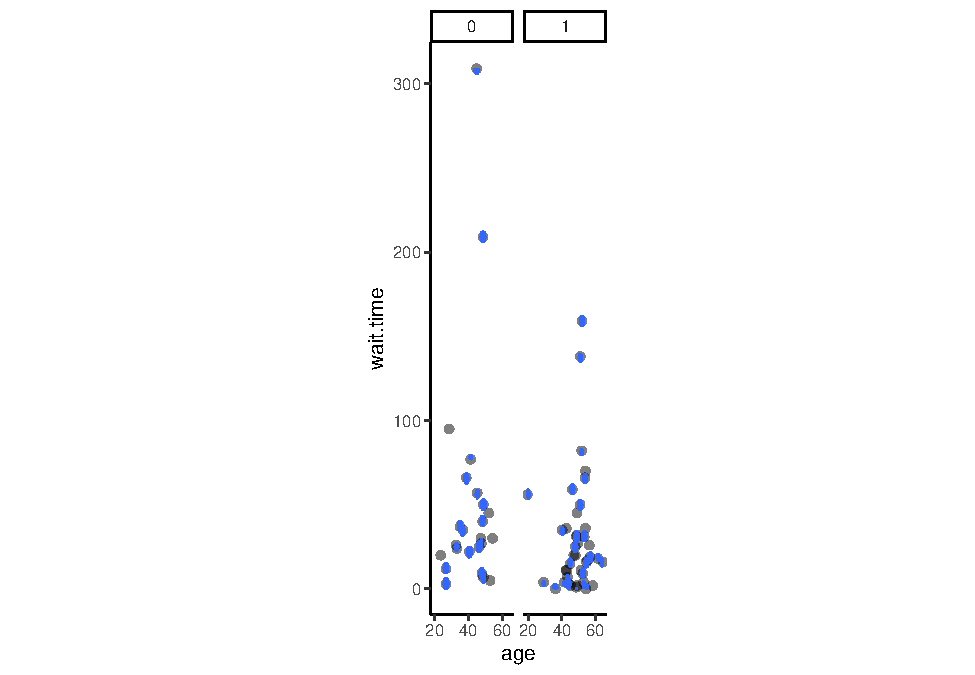
\includegraphics{proj2-2_files/figure-latex/unnamed-chunk-2-2} \end{center}

\begin{Shaded}
\begin{Highlighting}[]
\NormalTok{covmats<-jasa}\OperatorTok\KeywordTok{select}\NormalTok{(survive,age,reject,surgery,wait.time)}\OperatorTok\KeywordTok{group_by}\NormalTok{(survive)}\OperatorTok\KeywordTok{do}\NormalTok{(}\DataTypeTok{covs=}\KeywordTok{cov}\NormalTok{(.[}\DecValTok{2}\OperatorTok{:}\DecValTok{5}\NormalTok{]))}
\ControlFlowTok{for}\NormalTok{(i }\ControlFlowTok{in} \DecValTok{1}\OperatorTok{:}\DecValTok{3}\NormalTok{)\{}\KeywordTok{print}\NormalTok{(}\KeywordTok{as.character}\NormalTok{(covmats}\OperatorTok{$}\NormalTok{survive[i])); }\KeywordTok{print}\NormalTok{(covmats}\OperatorTok{$}\NormalTok{covs[i])\}}
\end{Highlighting}
\end{Shaded}

\begin{verbatim}
## [1] "0"
## [[1]]
##                  age reject    surgery  wait.time
## age       83.8716976      0  0.6213681   86.27593
## reject     0.0000000      0  0.0000000    0.00000
## surgery    0.6213681      0  0.2155797   -2.23913
## wait.time 86.2759277      0 -2.2391304 4777.73913
## 
## [1] "1"
## [[1]]
##                   age      reject     surgery   wait.time
## age       65.51982685  1.24270713 -0.04675882   20.075196
## reject     1.24270713  0.21219512 -0.01341463   -1.977439
## surgery   -0.04675882 -0.01341463  0.10975610    1.667683
## wait.time 20.07519574 -1.97743902  1.66768293 1181.230488
## 
## [1] NA
## [[1]]
## NULL
\end{verbatim}

\begin{Shaded}
\begin{Highlighting}[]
\NormalTok{man1<-}\KeywordTok{manova}\NormalTok{(}\KeywordTok{cbind}\NormalTok{(age,reject,surgery,wait.time)}\OperatorTok{~}\NormalTok{survive, }\DataTypeTok{data=}\NormalTok{jasa)}
\KeywordTok{summary}\NormalTok{(man1)}
\end{Highlighting}
\end{Shaded}

\begin{verbatim}
##           Df  Pillai approx F num Df den Df    Pr(>F)    
## survive    1 0.49649   14.791      4     60 1.826e-08 ***
## Residuals 63                                             
## ---
## Signif. codes:  0 '***' 0.001 '**' 0.01 '*' 0.05 '.' 0.1 ' ' 1
\end{verbatim}

\begin{Shaded}
\begin{Highlighting}[]
\KeywordTok{summary.aov}\NormalTok{(man1)}
\end{Highlighting}
\end{Shaded}

\begin{verbatim}
##  Response age :
##             Df Sum Sq Mean Sq F value   Pr(>F)   
## survive      1  752.1  752.14  10.415 0.001985 **
## Residuals   63 4549.8   72.22                    
## ---
## Signif. codes:  0 '***' 0.001 '**' 0.01 '*' 0.05 '.' 0.1 ' ' 1
## 
##  Response reject :
##             Df Sum Sq Mean Sq F value  Pr(>F)    
## survive      1 7.5737  7.5737  56.215 2.7e-10 ***
## Residuals   63 8.4878  0.1347                    
## ---
## Signif. codes:  0 '***' 0.001 '**' 0.01 '*' 0.05 '.' 0.1 ' ' 1
## 
##  Response surgery :
##             Df Sum Sq Mean Sq F value  Pr(>F)  
## survive      1 0.4360 0.43604  2.9385 0.09141 .
## Residuals   63 9.3486 0.14839                  
## ---
## Signif. codes:  0 '***' 0.001 '**' 0.01 '*' 0.05 '.' 0.1 ' ' 1
## 
##  Response wait.time :
##             Df Sum Sq Mean Sq F value  Pr(>F)  
## survive      1   7898  7898.2  3.1666 0.07998 .
## Residuals   63 157137  2494.2                  
## ---
## Signif. codes:  0 '***' 0.001 '**' 0.01 '*' 0.05 '.' 0.1 ' ' 1
\end{verbatim}

\begin{Shaded}
\begin{Highlighting}[]
\NormalTok{jasa}\OperatorTok\KeywordTok{group_by}\NormalTok{(survive)}\OperatorTok\KeywordTok{summarize}\NormalTok{(}\KeywordTok{mean}\NormalTok{(age),}\KeywordTok{mean}\NormalTok{(reject))}
\end{Highlighting}
\end{Shaded}

\begin{verbatim}
## # A tibble: 2 x 3
##   survive `mean(age)` `mean(reject)`
##     <dbl>       <dbl>          <dbl>
## 1       0        41.6          0    
## 2       1        48.6          0.707
\end{verbatim}

\begin{Shaded}
\begin{Highlighting}[]
\KeywordTok{pairwise.t.test}\NormalTok{(jasa}\OperatorTok{$}\NormalTok{age, jasa}\OperatorTok{$}\NormalTok{survive, }\DataTypeTok{p.adj =} \StringTok{"none"}\NormalTok{)}
\end{Highlighting}
\end{Shaded}

\begin{verbatim}
## 
##  Pairwise comparisons using t tests with pooled SD 
## 
## data:  jasa$age and jasa$survive 
## 
##   0    
## 1 0.002
## 
## P value adjustment method: none
\end{verbatim}

\begin{Shaded}
\begin{Highlighting}[]
\KeywordTok{pairwise.t.test}\NormalTok{(jasa}\OperatorTok{$}\NormalTok{reject, jasa}\OperatorTok{$}\NormalTok{survive, }\DataTypeTok{p.adj =} \StringTok{"none"}\NormalTok{)}
\end{Highlighting}
\end{Shaded}

\begin{verbatim}
## 
##  Pairwise comparisons using t tests with pooled SD 
## 
## data:  jasa$reject and jasa$survive 
## 
##   0      
## 1 2.7e-10
## 
## P value adjustment method: none
\end{verbatim}

\begin{Shaded}
\begin{Highlighting}[]
\DecValTok{1}\FloatTok{-.95}\OperatorTok{^}\NormalTok{(}\DecValTok{7}\NormalTok{) }\CommentTok{#error rate}
\end{Highlighting}
\end{Shaded}

\begin{verbatim}
## [1] 0.3016627
\end{verbatim}

\begin{Shaded}
\begin{Highlighting}[]
\FloatTok{0.05}\OperatorTok{/}\NormalTok{(}\DecValTok{7}\NormalTok{) }\CommentTok{#bonferroni corrections}
\end{Highlighting}
\end{Shaded}

\begin{verbatim}
## [1] 0.007142857
\end{verbatim}

\emph{After performing the MANOVA to determine differences in survival
with my dependent variables, the p value is less than 0.05, with an F
value of 14.791 which means there are mean differences across the levels
of survive (dead,1 or alive,0). When I performed univariate ANOVAs, I
found that the mean differences that were significant occur across age
and reject. I performed 1 MANOVA, 4 ANOVA, and 2 post hoc t tests. The
probability of type I error unadjusted is 30.16627\%. Adjusted according
to Bonferroni correction it is 0.007142857. Age and reject are still
significant after the correction. The significant differences in
survival were age of the patient and if they rejected the transplant.
Assumptions that were probably met were sample size because there are 65
observations, no extreme outliers, and no multicollinearity. Assumptions
that were not met are multivariate normality and homogeneity of
(co)variances because they are not similar across the groups and
multivariate normality of DVs.}

\hypertarget{randomization-test}{%
\paragraph{2. Randomization Test}\label{randomization-test}}

\begin{Shaded}
\begin{Highlighting}[]
\NormalTok{jasar<-jasa}\OperatorTok\KeywordTok{select}\NormalTok{(survive,age)}
\NormalTok{jasar}\OperatorTok\KeywordTok{group_by}\NormalTok{(survive)}\OperatorTok\KeywordTok{summarize}\NormalTok{(}\DataTypeTok{means=}\KeywordTok{mean}\NormalTok{(age))}\OperatorTok\KeywordTok{summarize}\NormalTok{(}\StringTok{`}\DataTypeTok{mean_diff:}\StringTok{`}\NormalTok{=}\KeywordTok{diff}\NormalTok{(means))}
\end{Highlighting}
\end{Shaded}

\begin{verbatim}
## # A tibble: 1 x 1
##   `mean_diff:`
##          <dbl>
## 1         7.05
\end{verbatim}

\begin{Shaded}
\begin{Highlighting}[]
\NormalTok{rand_dist<-}\KeywordTok{vector}\NormalTok{()}
\ControlFlowTok{for}\NormalTok{(i }\ControlFlowTok{in} \DecValTok{1}\OperatorTok{:}\DecValTok{5000}\NormalTok{)\{}
\NormalTok{new<-}\KeywordTok{data.frame}\NormalTok{(}\DataTypeTok{age=}\KeywordTok{sample}\NormalTok{(jasar}\OperatorTok{$}\NormalTok{age),}\DataTypeTok{survive=}\NormalTok{jasa}\OperatorTok{$}\NormalTok{survive)}
\NormalTok{rand_dist[i]<-}\KeywordTok{mean}\NormalTok{(new[new}\OperatorTok{$}\NormalTok{survive}\OperatorTok{==}\DecValTok{1}\NormalTok{,]}\OperatorTok{$}\NormalTok{age)}\OperatorTok{-}
\KeywordTok{mean}\NormalTok{(new[new}\OperatorTok{$}\NormalTok{survive}\OperatorTok{==}\DecValTok{0}\NormalTok{,]}\OperatorTok{$}\NormalTok{age)\}}
\KeywordTok{hist}\NormalTok{(rand_dist,}\DataTypeTok{main=}\StringTok{"Survival by Age"}\NormalTok{,}\DataTypeTok{ylab=}\StringTok{"Age"}\NormalTok{);}\KeywordTok{abline}\NormalTok{(}\DataTypeTok{v =} \FloatTok{7.0487}\NormalTok{ ,}\DataTypeTok{col=}\StringTok{"blue"}\NormalTok{); }\KeywordTok{abline}\NormalTok{(}\DataTypeTok{v =} \FloatTok{-7.0487}\NormalTok{    ,}\DataTypeTok{col=}\StringTok{"blue"}\NormalTok{)}
\end{Highlighting}
\end{Shaded}

\begin{center}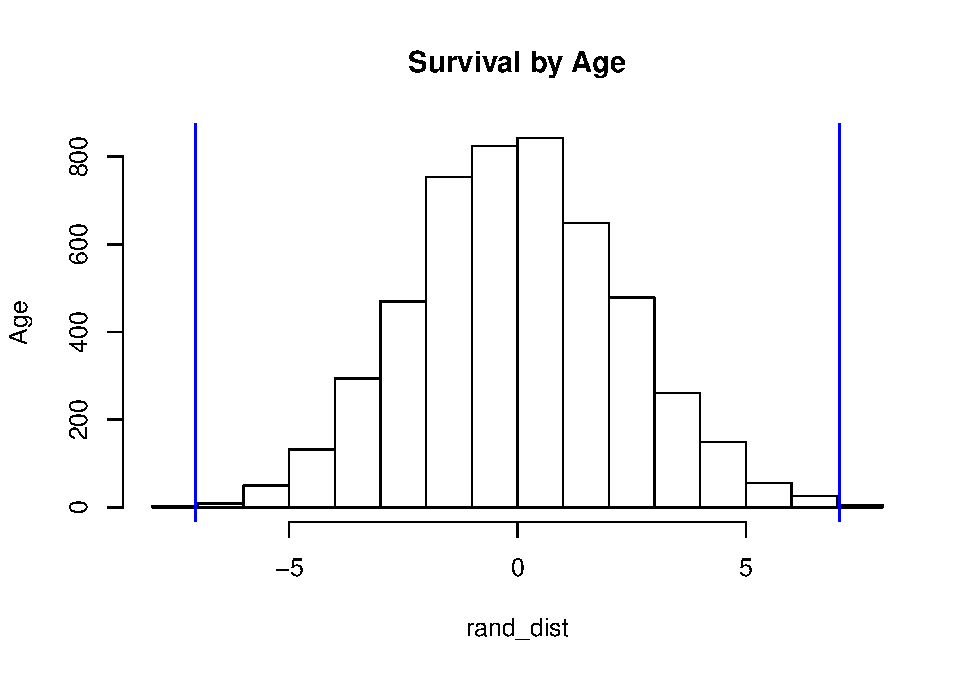
\includegraphics{proj2-2_files/figure-latex/unnamed-chunk-3-1} \end{center}

\begin{Shaded}
\begin{Highlighting}[]
\KeywordTok{mean}\NormalTok{(rand_dist}\OperatorTok{>}\FloatTok{7.0487}    \OperatorTok{|}\StringTok{ }\NormalTok{rand_dist}\OperatorTok{<}\StringTok{ }\FloatTok{-7.0487}\NormalTok{   )}
\end{Highlighting}
\end{Shaded}

\begin{verbatim}
## [1] 0.0012
\end{verbatim}

\begin{Shaded}
\begin{Highlighting}[]
\KeywordTok{ggplot}\NormalTok{(jasar,}\KeywordTok{aes}\NormalTok{(age,}\DataTypeTok{fill=}\NormalTok{survive))}\OperatorTok{+}\KeywordTok{geom_histogram}\NormalTok{(}\DataTypeTok{bins=}\FloatTok{6.5}\NormalTok{)}\OperatorTok{+}\KeywordTok{facet_wrap}\NormalTok{(}\OperatorTok{~}\NormalTok{survive,}\DataTypeTok{ncol=}\DecValTok{2}\NormalTok{)}\OperatorTok{+}\KeywordTok{theme}\NormalTok{(}\DataTypeTok{legend.position=}\StringTok{"none"}\OperatorTok{+}\KeywordTok{theme_classic}\NormalTok{())}
\end{Highlighting}
\end{Shaded}

\begin{center}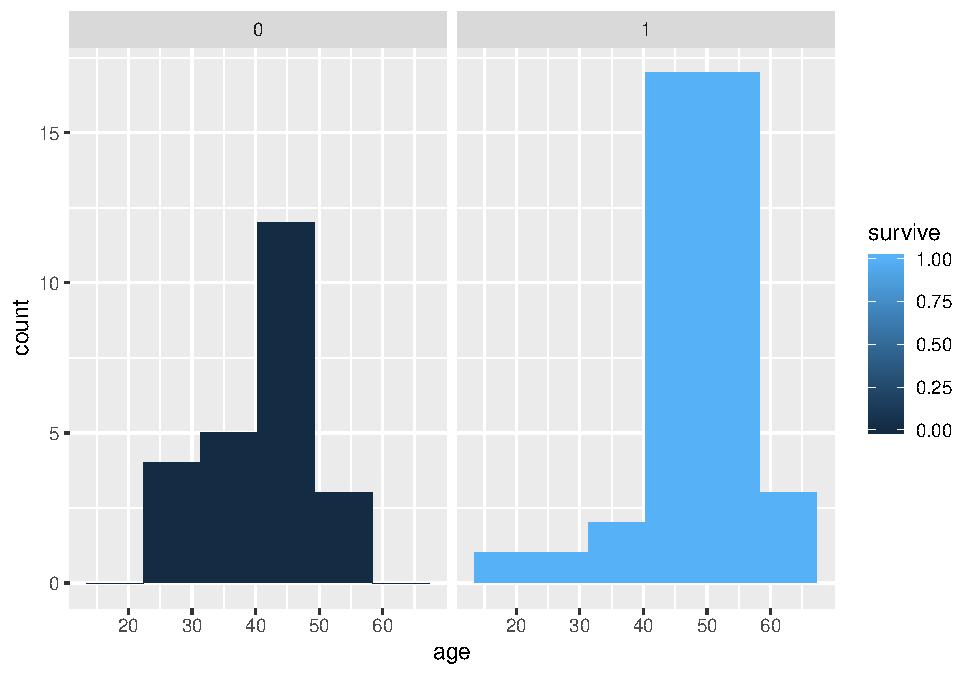
\includegraphics{proj2-2_files/figure-latex/unnamed-chunk-3-2} \end{center}

\emph{I used a randomization test in which the null hypothesis was that
mean age is the same for people that survived vs people that did not
survive surgery. The alternate hypothesis is that the mean age is
different for people that survived vs people that did not survive. The
two-tailed p value is 0.0012 so we can reject the null hypothesis. This
means the mean age is different for people that survived vs people that
did not survive.}

\hypertarget{linear-regression-model}{%
\paragraph{3. Linear Regression Model}\label{linear-regression-model}}

\begin{Shaded}
\begin{Highlighting}[]
\NormalTok{jasa}\OperatorTok{$}\NormalTok{wait.t_c<-jasa}\OperatorTok{$}\NormalTok{wait.time}\OperatorTok{-}\KeywordTok{mean}\NormalTok{(jasa}\OperatorTok{$}\NormalTok{wait.time)}
\NormalTok{fit<-}\KeywordTok{lm}\NormalTok{(age}\OperatorTok{~}\NormalTok{(reject}\OperatorTok{+}\NormalTok{surgery}\OperatorTok{+}\NormalTok{wait.t_c)}\OperatorTok{^}\DecValTok{2}\NormalTok{,}\DataTypeTok{data=}\NormalTok{jasa,}\DataTypeTok{family=}\StringTok{"binomial"}\NormalTok{)}
\KeywordTok{summary}\NormalTok{(fit) }
\end{Highlighting}
\end{Shaded}

\begin{verbatim}
## 
## Call:
## lm(formula = age ~ (reject + surgery + wait.t_c)^2, data = jasa, 
##     family = "binomial")
## 
## Residuals:
##      Min       1Q   Median       3Q      Max 
## -22.3021  -4.9398   0.2949   5.5796  15.4779 
## 
## Coefficients:
##                  Estimate Std. Error t value Pr(>|t|)    
## (Intercept)      41.61966    1.63295  25.487  < 2e-16 ***
## reject            9.15935    2.37888   3.850 0.000297 ***
## surgery           2.52725    3.50732   0.721 0.474073    
## wait.t_c          0.01303    0.02448   0.532 0.596498    
## reject:surgery   -5.16905    7.14623  -0.723 0.472387    
## reject:wait.t_c  -0.01077    0.06020  -0.179 0.858633    
## surgery:wait.t_c  0.04142    0.07543   0.549 0.585043    
## ---
## Signif. codes:  0 '***' 0.001 '**' 0.01 '*' 0.05 '.' 0.1 ' ' 1
## 
## Residual standard error: 8.452 on 58 degrees of freedom
## Multiple R-squared:  0.2186, Adjusted R-squared:  0.1378 
## F-statistic: 2.704 on 6 and 58 DF,  p-value: 0.02201
\end{verbatim}

\begin{Shaded}
\begin{Highlighting}[]
\KeywordTok{ggplot}\NormalTok{(jasa, }\KeywordTok{aes}\NormalTok{(}\DataTypeTok{x=}\NormalTok{wait.t_c, }\DataTypeTok{y=}\NormalTok{age,}\DataTypeTok{group=}\NormalTok{reject))}\OperatorTok{+}\KeywordTok{theme_classic}\NormalTok{()}\OperatorTok{+}\KeywordTok{geom_point}\NormalTok{(}\KeywordTok{aes}\NormalTok{(}\DataTypeTok{color=}\NormalTok{reject))}\OperatorTok{+}
\StringTok{  }\KeywordTok{geom_smooth}\NormalTok{(}\DataTypeTok{method=}\StringTok{"lm"}\NormalTok{,}\DataTypeTok{formula=}\NormalTok{y}\OperatorTok{~}\DecValTok{1}\NormalTok{,}\DataTypeTok{se=}\NormalTok{F,}\DataTypeTok{fullrange=}\NormalTok{T,}\KeywordTok{aes}\NormalTok{(}\DataTypeTok{color=}\NormalTok{reject))}\OperatorTok{+}
\KeywordTok{theme}\NormalTok{(}\DataTypeTok{legend.position=}\KeywordTok{c}\NormalTok{(.}\DecValTok{9}\NormalTok{,.}\DecValTok{25}\NormalTok{))}\OperatorTok{+}\KeywordTok{xlab}\NormalTok{(}\StringTok{"Wait.t_c"}\NormalTok{)}\OperatorTok{+}\KeywordTok{ggtitle}\NormalTok{(}\StringTok{"Linear Regression of Age with Wait Time and Rejection Status"}\NormalTok{)}
\end{Highlighting}
\end{Shaded}

\begin{center}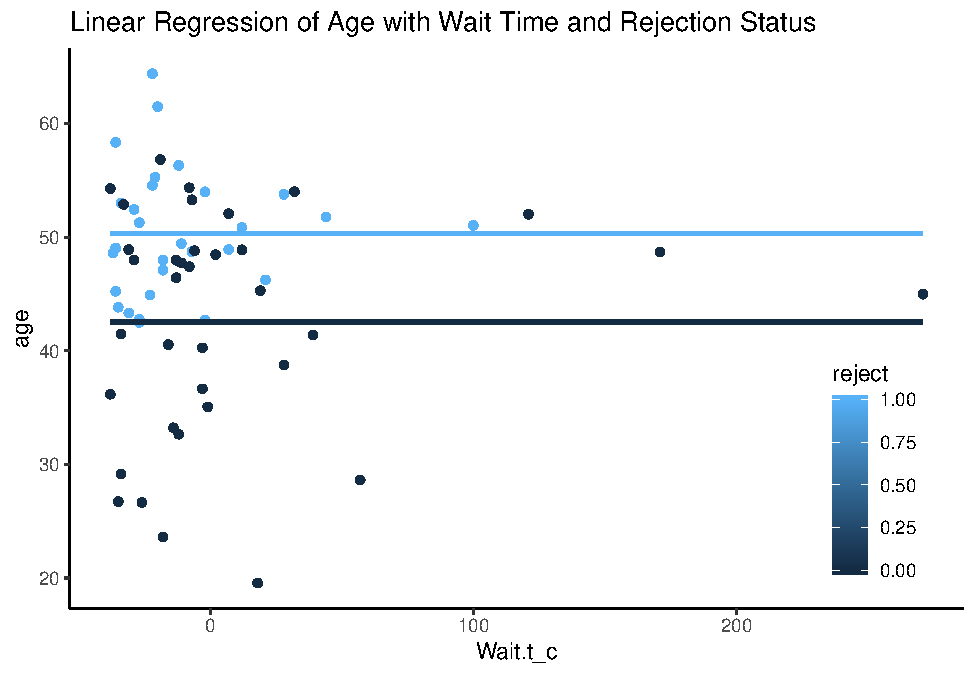
\includegraphics{proj2-2_files/figure-latex/unnamed-chunk-4-1} \end{center}

\begin{Shaded}
\begin{Highlighting}[]
\CommentTok{#linear relationships}
\NormalTok{resids<-fit}\OperatorTok{$}\NormalTok{residuals}
\NormalTok{fitvals<-fit}\OperatorTok{$}\NormalTok{fitted.values}
\KeywordTok{ggplot}\NormalTok{()}\OperatorTok{+}\KeywordTok{geom_point}\NormalTok{(}\KeywordTok{aes}\NormalTok{(fitvals,resids), }\DataTypeTok{color=}\StringTok{"blue"}\NormalTok{)}\OperatorTok{+}\KeywordTok{theme_classic}\NormalTok{()}
\end{Highlighting}
\end{Shaded}

\begin{center}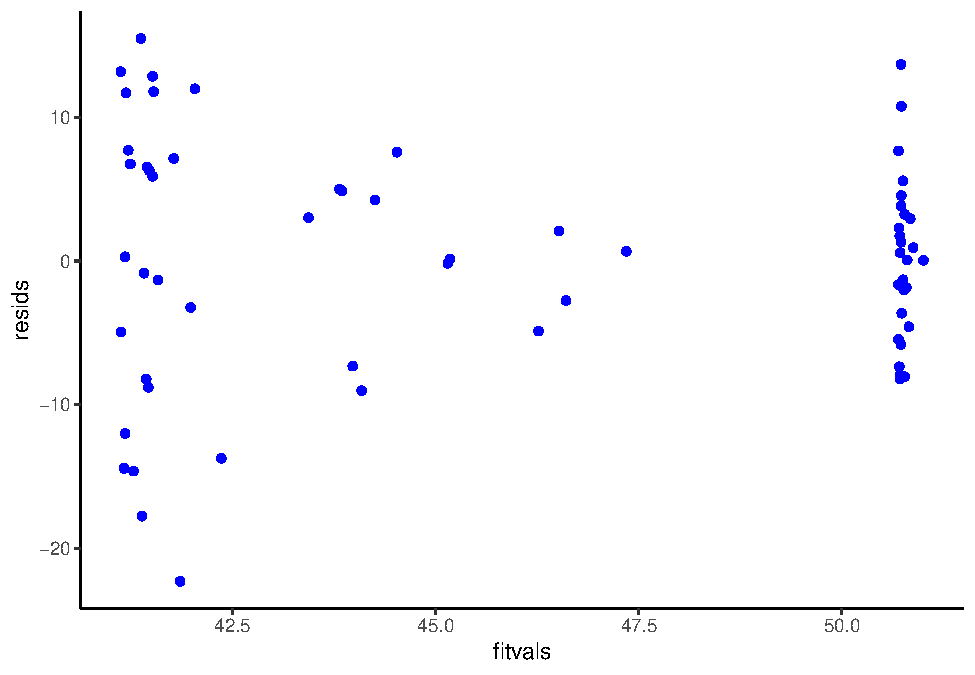
\includegraphics{proj2-2_files/figure-latex/unnamed-chunk-4-2} \end{center}

\begin{Shaded}
\begin{Highlighting}[]
\CommentTok{#normality }
\KeywordTok{shapiro.test}\NormalTok{(resids)}
\end{Highlighting}
\end{Shaded}

\begin{verbatim}
## 
##  Shapiro-Wilk normality test
## 
## data:  resids
## W = 0.98402, p-value = 0.5657
\end{verbatim}

\begin{Shaded}
\begin{Highlighting}[]
\CommentTok{#equal variance}
\KeywordTok{bptest}\NormalTok{(fit)}
\end{Highlighting}
\end{Shaded}

\begin{verbatim}
## 
##  studentized Breusch-Pagan test
## 
## data:  fit
## BP = 16.459, df = 6, p-value = 0.01149
\end{verbatim}

\begin{Shaded}
\begin{Highlighting}[]
\KeywordTok{coeftest}\NormalTok{(fit, }\DataTypeTok{vcov =} \KeywordTok{vcovHC}\NormalTok{(fit))[,}\DecValTok{1}\OperatorTok{:}\DecValTok{2}\NormalTok{] }
\end{Highlighting}
\end{Shaded}

\begin{verbatim}
##                     Estimate Std. Error
## (Intercept)      41.61966319 2.17949239
## reject            9.15935082 2.41279475
## surgery           2.52724593 3.32884133
## wait.t_c          0.01303268 0.01711262
## reject:surgery   -5.16904959 5.15002485
## reject:wait.t_c  -0.01076983 0.02790342
## surgery:wait.t_c  0.04141895 0.07740921
\end{verbatim}

\emph{When reject and surgery are 0 and wait time is the average, age is
41.620 years old. When reject is 1, the age goes up by 9.160 years, when
surgery is 1, the age goes up by 2.527 years, and when wait time is the
average, age goes up by 0.013 years. When you compare reject to surgery,
age goes down by 5.170 years. When you compare reject to average wait
time, age goes down by 0.011 years. When you compare surgery to average
wait time, age goes up by 0.041 years. Linearity looked to be supported.
Normality was supported. Equal variance was rejected with the BP test so
I corrected with robust SEs. The SEs increased for the intercept,
reject, wait.t\_c, and surgery:wait.t\_c. They decreased for surgery,
reject:surgery, and reject:wait.t\_c. My model explains 21.86\% of the
variation in the outcome.}

\hypertarget{linear-regression-model-with-bootstrapped-ses}{%
\paragraph{4. Linear Regression Model with Bootstrapped
SEs}\label{linear-regression-model-with-bootstrapped-ses}}

\begin{Shaded}
\begin{Highlighting}[]
\NormalTok{samp_distn<-}\KeywordTok{replicate}\NormalTok{(}\DecValTok{5000}\NormalTok{, \{}
\NormalTok{  boot_dat<-jasa[}\KeywordTok{sample}\NormalTok{(}\KeywordTok{nrow}\NormalTok{(jasa),}\DataTypeTok{replace=}\OtherTok{TRUE}\NormalTok{),]}
\NormalTok{  fit<-}\KeywordTok{lm}\NormalTok{(age}\OperatorTok{~}\NormalTok{(reject}\OperatorTok{+}\NormalTok{surgery}\OperatorTok{+}\NormalTok{wait.t_c)}\OperatorTok{^}\DecValTok{2}\NormalTok{, }\DataTypeTok{data=}\NormalTok{boot_dat) }
  \KeywordTok{coef}\NormalTok{(fit)\})}

\NormalTok{samp_distn}\OperatorTok\NormalTok{t}\OperatorTok\NormalTok{as.data.frame}\OperatorTok\KeywordTok{summarize_all}\NormalTok{(sd)}
\end{Highlighting}
\end{Shaded}

\begin{verbatim}
##   (Intercept)   reject  surgery   wait.t_c reject:surgery reject:wait.t_c
## 1    2.185032 2.405736 3.319769 0.04587252             NA      0.05481462
##   surgery:wait.t_c
## 1               NA
\end{verbatim}

\emph{The SEs in this bootstrapped model increased from all the robust
SEs. And different from the original SEs by increasing for the
intercept, reject, wait.t\_c, and reject:wait.t\_c, and decreased for
surgery.}

\hypertarget{logistic-regression-and-10-fold-cv}{%
\paragraph{5. Logistic Regression and 10-Fold
CV}\label{logistic-regression-and-10-fold-cv}}

\begin{Shaded}
\begin{Highlighting}[]
\NormalTok{jasa}\OperatorTok{$}\NormalTok{age_c<-jasa}\OperatorTok{$}\NormalTok{age}\OperatorTok{-}\KeywordTok{mean}\NormalTok{(jasa}\OperatorTok{$}\NormalTok{age)}
\NormalTok{jasa1<-jasa }\OperatorTok\KeywordTok{mutate}\NormalTok{(}\DataTypeTok{survive=}\KeywordTok{replace}\NormalTok{(survive, survive}\OperatorTok{==}\DecValTok{1}\NormalTok{, }\StringTok{"dead"}\NormalTok{),}\DataTypeTok{survive=}\KeywordTok{replace}\NormalTok{(survive, survive}\OperatorTok{==}\DecValTok{0}\NormalTok{, }\StringTok{"alive"}\NormalTok{)) }\OperatorTok\StringTok{ }\KeywordTok{as.data.frame}\NormalTok{()}

\NormalTok{data<-jasa1}\OperatorTok\KeywordTok{mutate}\NormalTok{(}\DataTypeTok{y=}\KeywordTok{ifelse}\NormalTok{(survive}\OperatorTok{==}\StringTok{"dead"}\NormalTok{,}\DecValTok{1}\NormalTok{,}\DecValTok{0}\NormalTok{))}
\NormalTok{outcome<-}\KeywordTok{factor}\NormalTok{(data}\OperatorTok{$}\NormalTok{survive,}\DataTypeTok{levels=}\KeywordTok{c}\NormalTok{(}\StringTok{"dead"}\NormalTok{,}\StringTok{"alive"}\NormalTok{))}

\NormalTok{fit1<-}\KeywordTok{glm}\NormalTok{(y}\OperatorTok{~}\NormalTok{age_c}\OperatorTok{+}\NormalTok{reject}\OperatorTok{+}\NormalTok{surgery}\OperatorTok{+}\NormalTok{wait.t_c, }\DataTypeTok{data=}\NormalTok{data,}\DataTypeTok{family=}\StringTok{"binomial"}\NormalTok{)}
\KeywordTok{coeftest}\NormalTok{(fit1)}
\end{Highlighting}
\end{Shaded}

\begin{verbatim}
## 
## z test of coefficients:
## 
##                Estimate  Std. Error z value Pr(>|z|)
## (Intercept) -3.6834e-01  4.2842e-01 -0.8598   0.3899
## age_c        3.9205e-02  3.8496e-02  1.0184   0.3085
## reject       1.9826e+01  1.9698e+03  0.0101   0.9920
## surgery     -7.7083e-01  9.1745e-01 -0.8402   0.4008
## wait.t_c    -5.2316e-03  7.1092e-03 -0.7359   0.4618
\end{verbatim}

\begin{Shaded}
\begin{Highlighting}[]
\KeywordTok{exp}\NormalTok{(}\KeywordTok{coef}\NormalTok{(fit1))}
\end{Highlighting}
\end{Shaded}

\begin{verbatim}
##  (Intercept)        age_c       reject      surgery     wait.t_c 
## 6.918853e-01 1.039984e+00 4.075661e+08 4.626275e-01 9.947821e-01
\end{verbatim}

\begin{Shaded}
\begin{Highlighting}[]
\NormalTok{probs<-}\KeywordTok{predict}\NormalTok{(fit1,}\DataTypeTok{type=}\StringTok{"response"}\NormalTok{)}
\KeywordTok{table}\NormalTok{(}\DataTypeTok{predict=}\KeywordTok{as.numeric}\NormalTok{(probs}\OperatorTok{>}\NormalTok{.}\DecValTok{5}\NormalTok{),}\DataTypeTok{truth=}\NormalTok{data}\OperatorTok{$}\NormalTok{y)}\OperatorTok\NormalTok{addmargins}
\end{Highlighting}
\end{Shaded}

\begin{verbatim}
##        truth
## predict  0  1 Sum
##     0   22 10  32
##     1    2 31  33
##     Sum 24 41  65
\end{verbatim}

\begin{Shaded}
\begin{Highlighting}[]
\NormalTok{class_diag<-}\ControlFlowTok{function}\NormalTok{(probs,truth)\{}
  \ControlFlowTok{if}\NormalTok{(}\KeywordTok{is.numeric}\NormalTok{(truth)}\OperatorTok{==}\OtherTok{FALSE} \OperatorTok{&}\StringTok{ }\KeywordTok{is.logical}\NormalTok{(truth)}\OperatorTok{==}\OtherTok{FALSE}\NormalTok{) truth<-}\KeywordTok{as.numeric}\NormalTok{(truth)}\OperatorTok{-}\DecValTok{1}
\NormalTok{  tab<-}\KeywordTok{table}\NormalTok{(}\KeywordTok{factor}\NormalTok{(probs}\OperatorTok{>}\NormalTok{.}\DecValTok{5}\NormalTok{,}\DataTypeTok{levels=}\KeywordTok{c}\NormalTok{(}\StringTok{"FALSE"}\NormalTok{,}\StringTok{"TRUE"}\NormalTok{)),truth)}
\NormalTok{  prediction<-}\KeywordTok{ifelse}\NormalTok{(probs}\OperatorTok{>}\NormalTok{.}\DecValTok{5}\NormalTok{,}\DecValTok{1}\NormalTok{,}\DecValTok{0}\NormalTok{)}
\NormalTok{  acc=}\KeywordTok{mean}\NormalTok{(truth}\OperatorTok{==}\NormalTok{prediction)}
\NormalTok{  sens=}\KeywordTok{mean}\NormalTok{(prediction[truth}\OperatorTok{==}\DecValTok{1}\NormalTok{]}\OperatorTok{==}\DecValTok{1}\NormalTok{)}
\NormalTok{  spec=}\KeywordTok{mean}\NormalTok{(prediction[truth}\OperatorTok{==}\DecValTok{0}\NormalTok{]}\OperatorTok{==}\DecValTok{0}\NormalTok{)}
\NormalTok{  ppv=}\KeywordTok{mean}\NormalTok{(truth[prediction}\OperatorTok{==}\DecValTok{1}\NormalTok{]}\OperatorTok{==}\DecValTok{1}\NormalTok{)}
\NormalTok{  ord<-}\KeywordTok{order}\NormalTok{(probs, }\DataTypeTok{decreasing=}\OtherTok{TRUE}\NormalTok{)}
\NormalTok{  probs <-}\StringTok{ }\NormalTok{probs[ord]; truth <-}\StringTok{ }\NormalTok{truth[ord]}
\NormalTok{  TPR=}\KeywordTok{cumsum}\NormalTok{(truth)}\OperatorTok{/}\KeywordTok{max}\NormalTok{(}\DecValTok{1}\NormalTok{,}\KeywordTok{sum}\NormalTok{(truth)) }
\NormalTok{  FPR=}\KeywordTok{cumsum}\NormalTok{(}\OperatorTok{!}\NormalTok{truth)}\OperatorTok{/}\KeywordTok{max}\NormalTok{(}\DecValTok{1}\NormalTok{,}\KeywordTok{sum}\NormalTok{(}\OperatorTok{!}\NormalTok{truth))}
\NormalTok{  dup<-}\KeywordTok{c}\NormalTok{(probs[}\OperatorTok{-}\DecValTok{1}\NormalTok{]}\OperatorTok{>=}\NormalTok{probs[}\OperatorTok{-}\KeywordTok{length}\NormalTok{(probs)], }\OtherTok{FALSE}\NormalTok{)}
\NormalTok{  TPR<-}\KeywordTok{c}\NormalTok{(}\DecValTok{0}\NormalTok{,TPR[}\OperatorTok{!}\NormalTok{dup],}\DecValTok{1}\NormalTok{); FPR<-}\KeywordTok{c}\NormalTok{(}\DecValTok{0}\NormalTok{,FPR[}\OperatorTok{!}\NormalTok{dup],}\DecValTok{1}\NormalTok{)}
\NormalTok{  n <-}\StringTok{ }\KeywordTok{length}\NormalTok{(TPR)}
\NormalTok{  auc<-}\StringTok{ }\KeywordTok{sum}\NormalTok{( ((TPR[}\OperatorTok{-}\DecValTok{1}\NormalTok{]}\OperatorTok{+}\NormalTok{TPR[}\OperatorTok{-}\NormalTok{n])}\OperatorTok{/}\DecValTok{2}\NormalTok{) }\OperatorTok{*}\StringTok{ }\NormalTok{(FPR[}\OperatorTok{-}\DecValTok{1}\NormalTok{]}\OperatorTok{-}\NormalTok{FPR[}\OperatorTok{-}\NormalTok{n]) )}
\KeywordTok{data.frame}\NormalTok{(acc,sens,spec,ppv,auc)\}}
\KeywordTok{class_diag}\NormalTok{(probs,data}\OperatorTok{$}\NormalTok{y)}
\end{Highlighting}
\end{Shaded}

\begin{verbatim}
##         acc      sens      spec       ppv       auc
## 1 0.8153846 0.7560976 0.9166667 0.9393939 0.8973577
\end{verbatim}

\begin{Shaded}
\begin{Highlighting}[]
\NormalTok{data}\OperatorTok{$}\NormalTok{logit<-}\KeywordTok{predict}\NormalTok{(fit1,}\DataTypeTok{type=}\StringTok{"link"}\NormalTok{)}
\NormalTok{data}\OperatorTok\KeywordTok{ggplot}\NormalTok{()}\OperatorTok{+}\KeywordTok{geom_density}\NormalTok{(}\KeywordTok{aes}\NormalTok{(logit,}\DataTypeTok{color=}\NormalTok{outcome,}\DataTypeTok{fill=}\NormalTok{outcome), }\DataTypeTok{alpha=}\NormalTok{.}\DecValTok{4}\NormalTok{)}\OperatorTok{+}
\StringTok{  }\KeywordTok{theme_classic}\NormalTok{()}\OperatorTok{+}\KeywordTok{geom_vline}\NormalTok{(}\DataTypeTok{xintercept=}\DecValTok{0}\NormalTok{)}\OperatorTok{+}\KeywordTok{xlab}\NormalTok{(}\StringTok{"logit (log-odds)"}\NormalTok{)}\OperatorTok{+}
\StringTok{  }\KeywordTok{geom_rug}\NormalTok{(}\KeywordTok{aes}\NormalTok{(logit,}\DataTypeTok{color=}\NormalTok{outcome))}\OperatorTok{+}
\StringTok{  }\KeywordTok{geom_text}\NormalTok{(}\DataTypeTok{x=}\OperatorTok{-}\DecValTok{5}\NormalTok{,}\DataTypeTok{y=}\NormalTok{.}\DecValTok{07}\NormalTok{,}\DataTypeTok{label=}\StringTok{"TN = 31"}\NormalTok{)}\OperatorTok{+}
\StringTok{  }\KeywordTok{geom_text}\NormalTok{(}\DataTypeTok{x=}\OperatorTok{-}\FloatTok{1.75}\NormalTok{,}\DataTypeTok{y=}\NormalTok{.}\DecValTok{008}\NormalTok{,}\DataTypeTok{label=}\StringTok{"FN = 10"}\NormalTok{)}\OperatorTok{+}
\StringTok{  }\KeywordTok{geom_text}\NormalTok{(}\DataTypeTok{x=}\DecValTok{1}\NormalTok{,}\DataTypeTok{y=}\NormalTok{.}\DecValTok{006}\NormalTok{,}\DataTypeTok{label=}\StringTok{"FP = 2"}\NormalTok{)}\OperatorTok{+}
\StringTok{  }\KeywordTok{geom_text}\NormalTok{(}\DataTypeTok{x=}\DecValTok{5}\NormalTok{,}\DataTypeTok{y=}\NormalTok{.}\DecValTok{04}\NormalTok{,}\DataTypeTok{label=}\StringTok{"TP = 22"}\NormalTok{)}
\end{Highlighting}
\end{Shaded}

\begin{center}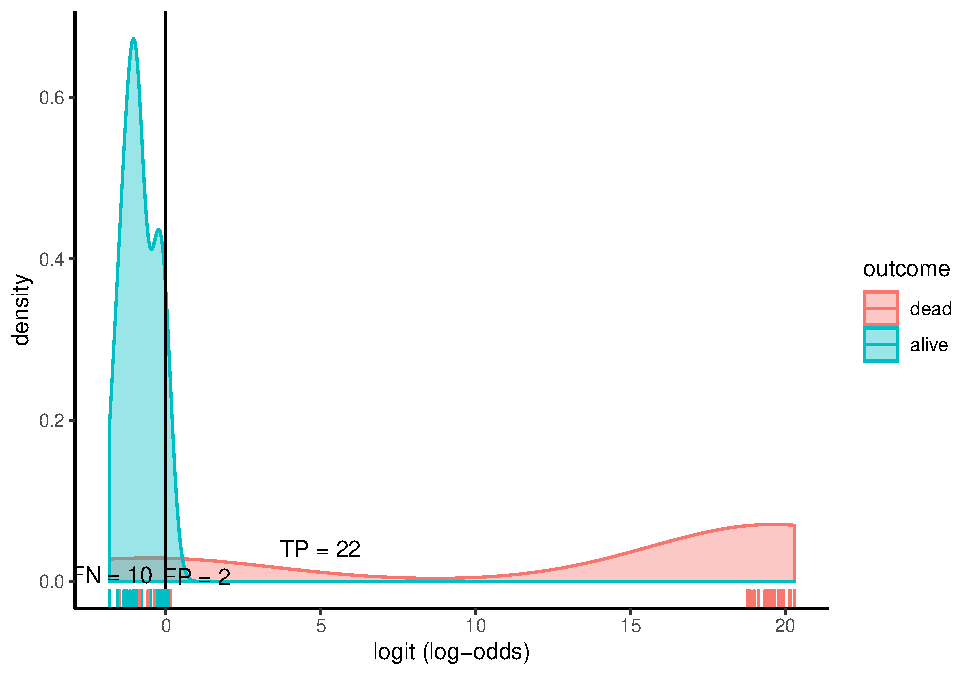
\includegraphics{proj2-2_files/figure-latex/unnamed-chunk-6-1} \end{center}

\begin{Shaded}
\begin{Highlighting}[]
\NormalTok{ROCplot<-}\KeywordTok{ggplot}\NormalTok{(data)}\OperatorTok{+}\KeywordTok{geom_roc}\NormalTok{(}\KeywordTok{aes}\NormalTok{(}\DataTypeTok{d=}\NormalTok{y,}\DataTypeTok{m=}\NormalTok{probs), }\DataTypeTok{n.cuts=}\DecValTok{0}\NormalTok{)}\OperatorTok{+}\KeywordTok{theme_classic}\NormalTok{()}
\NormalTok{ROCplot}
\end{Highlighting}
\end{Shaded}

\begin{center}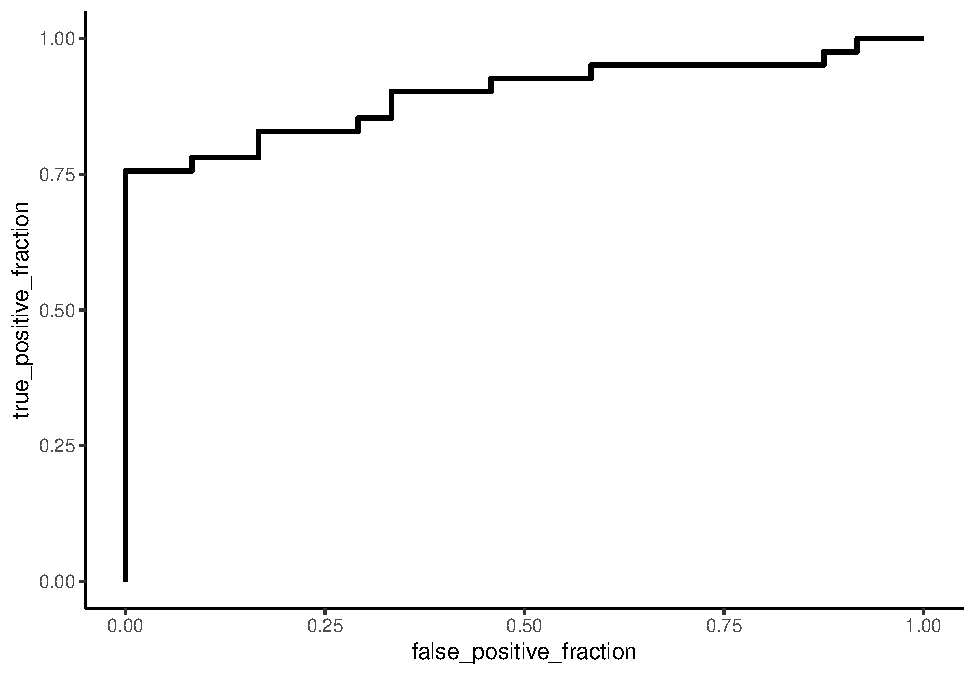
\includegraphics{proj2-2_files/figure-latex/unnamed-chunk-6-2} \end{center}

\begin{Shaded}
\begin{Highlighting}[]
\KeywordTok{calc_auc}\NormalTok{(ROCplot)}
\end{Highlighting}
\end{Shaded}

\begin{verbatim}
##   PANEL group       AUC
## 1     1    -1 0.8973577
\end{verbatim}

\begin{Shaded}
\begin{Highlighting}[]
\KeywordTok{set.seed}\NormalTok{(}\DecValTok{1234}\NormalTok{)}
\NormalTok{k=}\DecValTok{10}
\NormalTok{data1<-data[}\KeywordTok{sample}\NormalTok{(}\KeywordTok{nrow}\NormalTok{(data)),] }
\NormalTok{folds<-}\KeywordTok{cut}\NormalTok{(}\KeywordTok{seq}\NormalTok{(}\DecValTok{1}\OperatorTok{:}\KeywordTok{nrow}\NormalTok{(data)),}\DataTypeTok{breaks=}\NormalTok{k,}\DataTypeTok{labels=}\NormalTok{F) }
\NormalTok{diags<-}\OtherTok{NULL}
\ControlFlowTok{for}\NormalTok{(i }\ControlFlowTok{in} \DecValTok{1}\OperatorTok{:}\NormalTok{k)\{         }
\NormalTok{  train<-data[folds}\OperatorTok{!=}\NormalTok{i,] }
\NormalTok{  test<-data[folds}\OperatorTok{==}\NormalTok{i,]  }
\NormalTok{  truth<-test}\OperatorTok{$}\NormalTok{y}
\NormalTok{  fit<-}\KeywordTok{glm}\NormalTok{(y}\OperatorTok{~}\NormalTok{age_c}\OperatorTok{+}\NormalTok{reject}\OperatorTok{+}\NormalTok{surgery}\OperatorTok{+}\NormalTok{wait.t_c,}\DataTypeTok{data=}\NormalTok{train,}\DataTypeTok{family=}\StringTok{"binomial"}\NormalTok{)}
\NormalTok{  probs<-}\KeywordTok{predict}\NormalTok{(fit,}\DataTypeTok{newdata =}\NormalTok{ test,}\DataTypeTok{type=}\StringTok{"response"}\NormalTok{)}
\NormalTok{  diags<-}\KeywordTok{rbind}\NormalTok{(diags,}\KeywordTok{class_diag}\NormalTok{(probs,truth)) \}}
\KeywordTok{summarize_all}\NormalTok{(diags,mean) }
\end{Highlighting}
\end{Shaded}

\begin{verbatim}
##         acc      sens spec       ppv       auc
## 1 0.7642857 0.7571429  NaN 0.9016667 0.8583333
\end{verbatim}

\emph{When a person is at the average age, the odds that they died is
1.03. When reject is 0 the odds that they died are 407566106. When
surgery is 0 the odds that they died is -0.77. When a person has an
average wait time the odds that they died is -0.005. There were 22 true
positives, 31 true negatives, 2 false positives, and 10 false negatives.
The AUC is 0.897 so it is a great tradeoff between sensitivity and
specificity for my data. When you use a 10-fold CV it goes down to
0.858, so there is evidence of overfitting. The average out-of-sample
accuracy is 0.814, the sensitivity is 0.755, and the recall is 0.925.}

\hypertarget{lasso-and-10-fold-cv}{%
\paragraph{6. LASSO and 10-Fold CV}\label{lasso-and-10-fold-cv}}

\begin{Shaded}
\begin{Highlighting}[]
\KeywordTok{set.seed}\NormalTok{(}\DecValTok{1234}\NormalTok{)}
\NormalTok{y<-}\KeywordTok{as.matrix}\NormalTok{(data}\OperatorTok{$}\NormalTok{y) }\CommentTok{#grab response}
\NormalTok{x<-}\KeywordTok{model.matrix}\NormalTok{(y}\OperatorTok{~}\NormalTok{age_c}\OperatorTok{+}\NormalTok{reject}\OperatorTok{+}\NormalTok{surgery}\OperatorTok{+}\NormalTok{wait.t_c,}\DataTypeTok{data=}\NormalTok{data)[,}\OperatorTok{-}\DecValTok{1}\NormalTok{]}
\NormalTok{cv <-}\StringTok{ }\KeywordTok{cv.glmnet}\NormalTok{(x,y)}
\NormalTok{cv<-}\KeywordTok{cv.glmnet}\NormalTok{(x,y,}\DataTypeTok{family=}\StringTok{"binomial"}\NormalTok{)}
\NormalTok{lasso<-}\KeywordTok{glmnet}\NormalTok{(x,y,}\DataTypeTok{family=}\StringTok{"binomial"}\NormalTok{,}\DataTypeTok{lambda=}\NormalTok{cv}\OperatorTok{$}\NormalTok{lambda}\FloatTok{.1}\NormalTok{se)}
\KeywordTok{coef}\NormalTok{(lasso)}
\end{Highlighting}
\end{Shaded}

\begin{verbatim}
## 5 x 1 sparse Matrix of class "dgCMatrix"
##                    s0
## (Intercept) -0.151940
## age_c        .       
## reject       1.811409
## surgery      .       
## wait.t_c     .
\end{verbatim}

\begin{Shaded}
\begin{Highlighting}[]
\KeywordTok{set.seed}\NormalTok{(}\DecValTok{1234}\NormalTok{)}
\NormalTok{k=}\DecValTok{10}
\NormalTok{data <-}\StringTok{ }\NormalTok{data}\OperatorTok\StringTok{ }\NormalTok{sample_frac }\CommentTok{#put rows of dataset in random order}
\NormalTok{folds <-}\StringTok{ }\KeywordTok{ntile}\NormalTok{(}\DecValTok{1}\OperatorTok{:}\KeywordTok{nrow}\NormalTok{(data),}\DataTypeTok{n=}\DecValTok{10}\NormalTok{) }\CommentTok{#create fold labels}
\NormalTok{diags<-}\OtherTok{NULL}
\ControlFlowTok{for}\NormalTok{(i }\ControlFlowTok{in} \DecValTok{1}\OperatorTok{:}\NormalTok{k)\{}
\NormalTok{train <-}\StringTok{ }\NormalTok{data[folds}\OperatorTok{!=}\NormalTok{i,] }\CommentTok{#create training set (all but fold i)}
\NormalTok{test <-}\StringTok{ }\NormalTok{data[folds}\OperatorTok{==}\NormalTok{i,] }\CommentTok{#create test set (just fold i)}
\NormalTok{truth <-}\StringTok{ }\NormalTok{test}\OperatorTok{$}\NormalTok{y }\CommentTok{#save truth labels from fold i}
\NormalTok{fit <-}\StringTok{ }\KeywordTok{glm}\NormalTok{(y}\OperatorTok{~}\NormalTok{reject,}
\DataTypeTok{data=}\NormalTok{train, }\DataTypeTok{family=}\StringTok{"binomial"}\NormalTok{)}
\NormalTok{probs <-}\StringTok{ }\KeywordTok{predict}\NormalTok{(fit, }\DataTypeTok{newdata=}\NormalTok{test, }\DataTypeTok{type=}\StringTok{"response"}\NormalTok{)}
\NormalTok{diags<-}\KeywordTok{rbind}\NormalTok{(diags,}\KeywordTok{class_diag}\NormalTok{(probs,truth))}
\NormalTok{\}}
\NormalTok{diags}\OperatorTok\KeywordTok{summarize_all}\NormalTok{(mean)}
\end{Highlighting}
\end{Shaded}

\begin{verbatim}
##         acc sens spec ppv   auc
## 1 0.8142857 0.69    1   1 0.845
\end{verbatim}

\emph{When I used a LASSO, the only variable maintained is reject which
makes sense. If someone rejects their transplant they are more likely to
die. When I ran a 10-fold CV with just reject the accuracy went up from
0.762 to 0.0814.}

\#\#\#Sources

\emph{{[}1{]} John Crowley \& Marie Hu (1977) Covariance Analysis of
Heart Transplant Survival Data, Journal of the American Statistical
Association, 72:357, 27-36} \ldots{}

\end{document}
